%%%%%%%%%%%%%%%%%%%%%%%%%%%%%%%%%%%%%%
%%%%%%%%%%%%%%%%%%%%%%%%%%%%%%%%%%%%%%
% Do not edit the TeX file your work
% will be overwritten.  Edit the RnW
% file instead.
%%%%%%%%%%%%%%%%%%%%%%%%%%%%%%%%%%%%%%
%%%%%%%%%%%%%%%%%%%%%%%%%%%%%%%%%%%%%%



We consider the problem of clustering time-course gene expression data. 
While thousands genes might be measured in a given genomics experiment, 
many genes may exhibit similar expression patterns.  
Clustering genes is one way to reduce the dimensionality of a complex data set 
and faciliates scientific interpretations. 
Often, such dimensionality reduction is used for exploratory analysis and
is a first step before further downstream analyses. 
It is important, therefore, to acertain the stability of the 
discovered clusters. 
 
We study a publicly available data set of mice gene expression
\citep{shoemaker:2015:ultrasensitive}.
Mice were infected with different influenza viruses, and gene expression
was assessed at 14 time points after infection.
Our analysis focuses on mice treated with the ``A/California/04/2009'' strain. 
We normalize the data as described in
\citet{shoemaker:2015:ultrasensitive} and then apply the differential
analysis tool EDGE \citep{Storey:2005:significance} to rank the genes from most to least significantly differentially expressed. 
We run our analysis below on the top $\ngenes = 1000$ genes.

\subsubsection*{The model}


Each gene consists of $\ntimepoints = 42$ measurements of expression: three replicates at 14 unique timepoints.
The timepoints are unevenly spaced, with more frequent observations at the beginning. 
We model the first 11 timepoints with cubic B-splines with 7 degrees of freedom.
For the last three timepoints, $t = 72, 120, 168$ hours,
we use indicator functions. 
That is, if $\tilde X$ is the matrix where each column is a B-spline basis vector evaluated at the $\ntimepoints$ timepoints, we append to $\tilde X$ three additional columns where each column is 1 if $t = 72, 120,$ or 168, repectively, and 0 otherwise. 
Call the full design matrix $X$. 
Without the indicator columns, the matrix $\tilde X^T \tilde X$ is nearly singular, because the later timepoints are more spread out. 
See \figref{example_genes} for an example gene and the B-spline basis. 

Let $\x_\n$ be the vector of observations $(\x_{\n 1}, ..., \x_{\n \ntimepoints})^T$.
Each cluster is characterized by a vector of regression coefficients 
$\theta_k$; the distribution of the data arising from cluster $k$ is 
\begin{align*}
p(\x_\n | \theta_k, b_{n}) = \normdist{\x_\n | X\theta_k + b_{n}, \sigma^2I_{M \times M}},
\end{align*}
where $b_{n}$ is a gene-specific additive offset. 

The joint distribution similar to~\eqref{bnp_model}, except with the addition of the additive offset: 
\begin{align*}
\MoveEqLeft
\logp(\x, \theta, \z, \nu) ={}
\nonumber\\&
    \sum_{n=1}^N \sum_{k=1}^{\kmax}
        \z_{\n\k} \left(
            \logp(\x_n \vert \theta_\k, b_n) + \logp(b_n) \log \pi_\k
        \right) +
    \sum_{k=1}^{\kmax} \left(
        \log \pstick(\nuk) + \logp(\theta_\k)
    \right).
\end{align*}

%

\begin{knitrout}
\definecolor{shadecolor}{rgb}{0.969, 0.969, 0.969}\color{fgcolor}\begin{figure}[!h]

{\centering 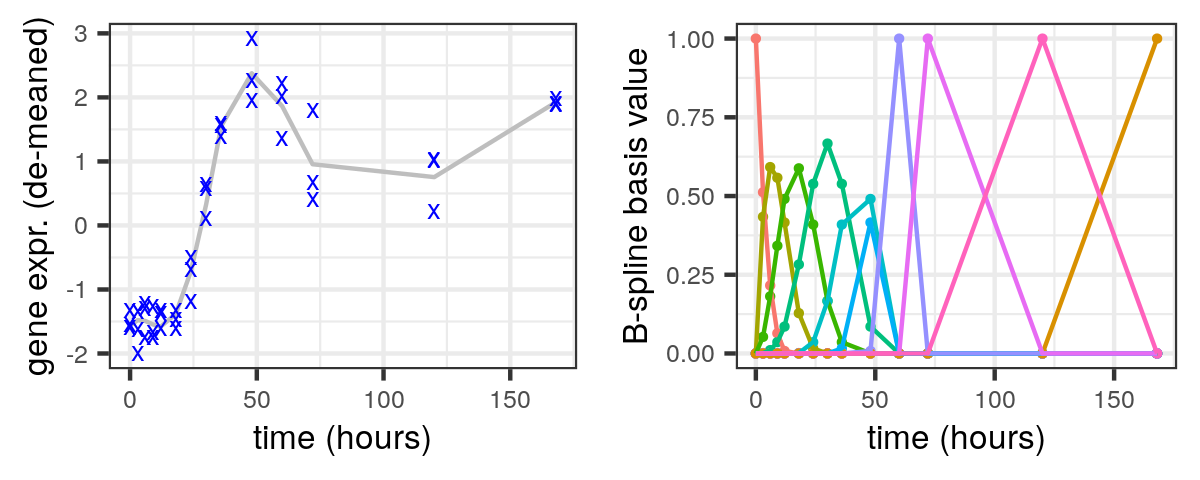
\includegraphics[width=0.980\linewidth,height=0.392\linewidth]{figure/example_genes-1} 

}

\caption[(Left) An example gene and its expression over time.
     (Right) The cubic B-spline with 7 degrees of freedom]{(Left) An example gene and its expression over time.
     (Right) The cubic B-spline with 7 degrees of freedom. }\label{fig:example_genes}
\end{figure}


\end{knitrout}
%






\begin{knitrout}
\definecolor{shadecolor}{rgb}{0.969, 0.969, 0.969}\color{fgcolor}\begin{figure}[!h]

{\centering 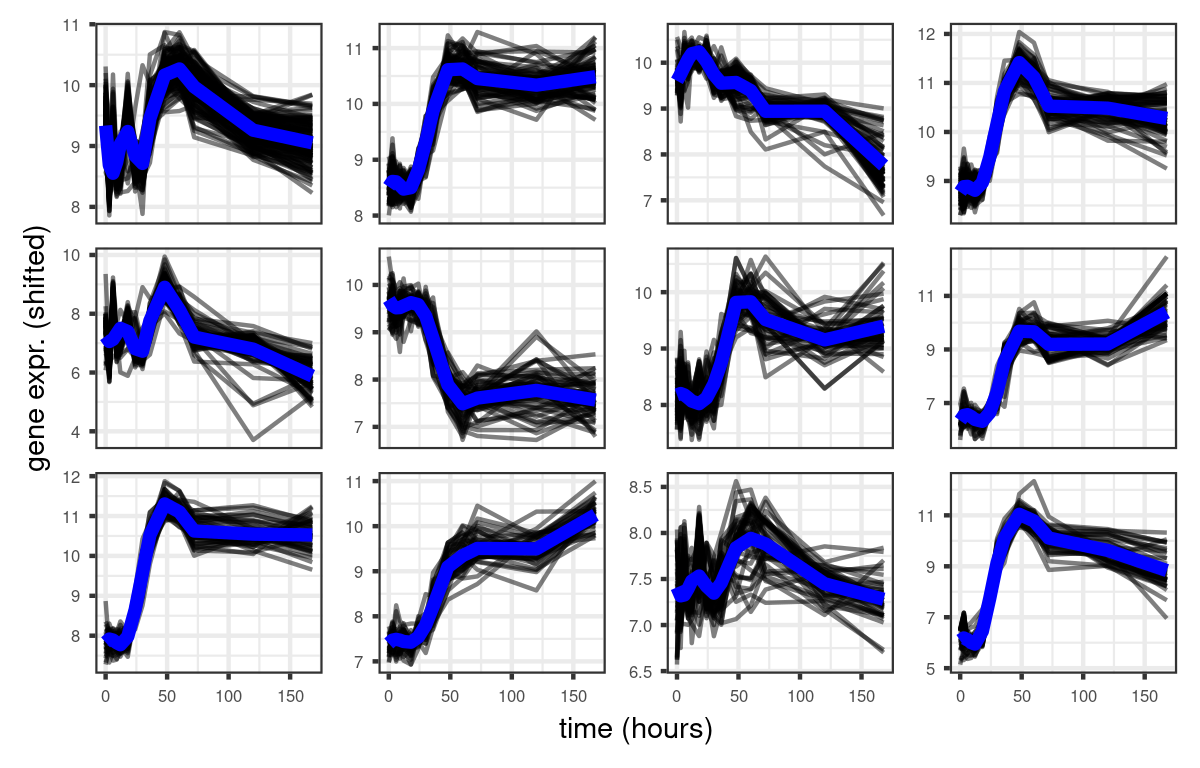
\includegraphics[width=0.980\linewidth,height=0.627\linewidth]{figure/gene_centroids-1} 

}

\caption[In blue, inferred centroids from the twelve most occupied clusters.
    In grey, gene expressions averaged over replicates and
    shifted by their inferred intercepts]{In blue, inferred centroids from the twelve most occupied clusters.
    In grey, gene expressions averaged over replicates and
    shifted by their inferred intercepts. }\label{fig:gene_centroids}
\end{figure}


\end{knitrout}







\begin{knitrout}
\definecolor{shadecolor}{rgb}{0.969, 0.969, 0.969}\color{fgcolor}\begin{figure}[!h]

{\centering 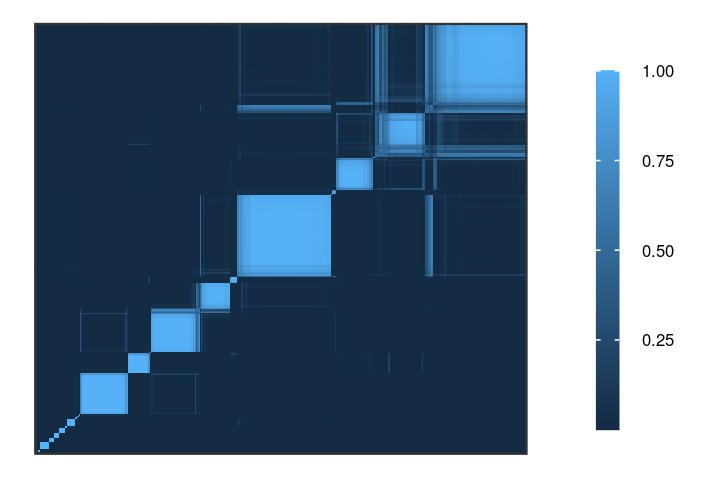
\includegraphics[width=0.588\linewidth,height=0.400\linewidth]{figure/gene_initial_coclustering-1} 

}

\caption[The inferred co-clustering of gene expressions at $\alpha = 3.$ ]{The inferred co-clustering of gene expressions at $\alpha = 3.$ }\label{fig:gene_initial_coclustering}
\end{figure}


\end{knitrout}










\begin{knitrout}
\definecolor{shadecolor}{rgb}{0.969, 0.969, 0.969}\color{fgcolor}\begin{figure}[!h]

{\centering 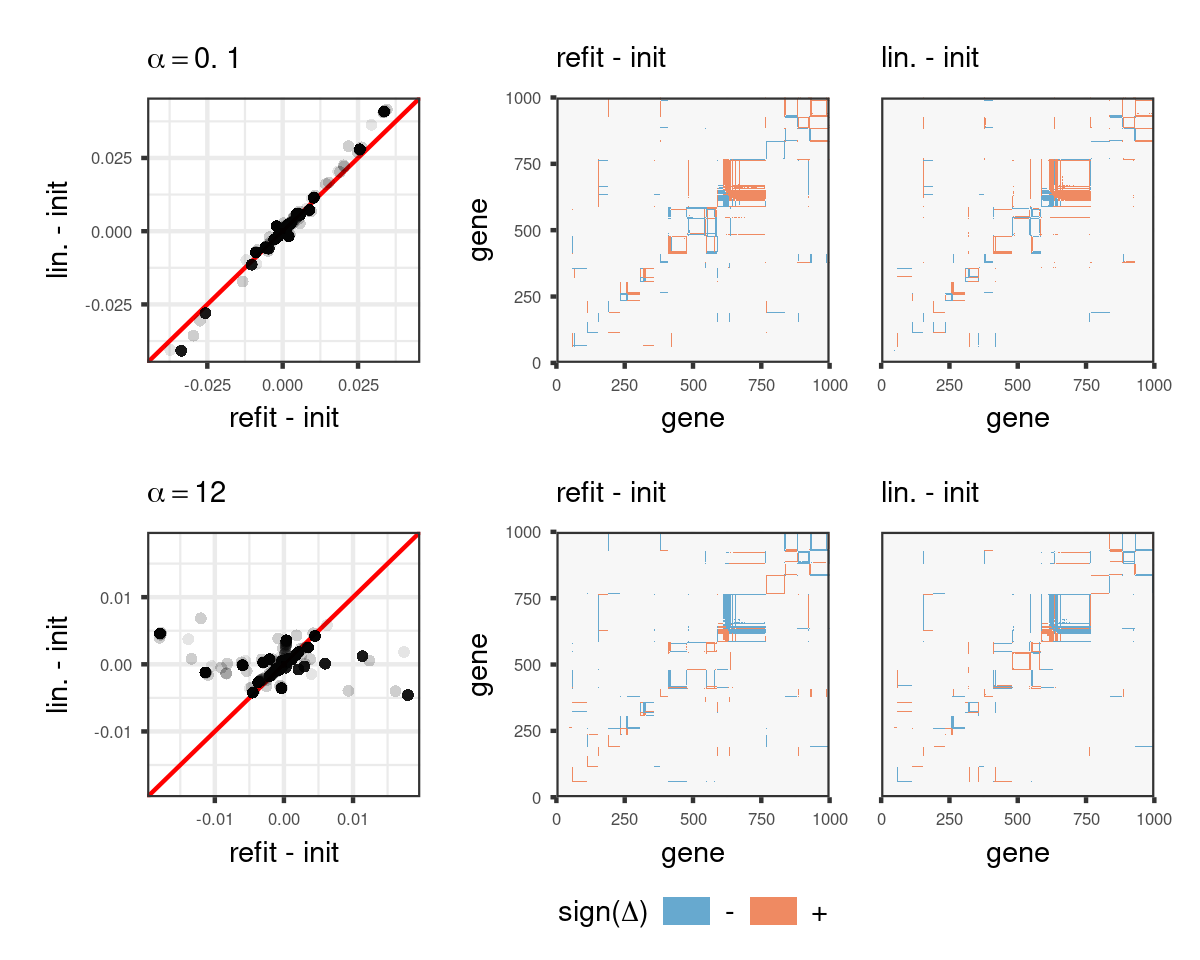
\includegraphics[width=0.980\linewidth,height=0.784\linewidth]{figure/gene_alpha_coclustering-1} 

}

\caption[Changes in the co-clustering matrix at alpha = 1 (top row)
     and alpha = 11 (bottom row),
     relative to the co-clustering matrix at alpha = 3.
     The left column plots differences predicted by the
     linear approximation against differences from a model refit.
     Each point represents an entry of the co-coclustering matrix.
     The middle and right columns display
     changes in the co-clustering matrix as obtained by the
     linear approximation and the model refit, respectively]{Changes in the co-clustering matrix at alpha = 1 (top row)
     and alpha = 11 (bottom row),
     relative to the co-clustering matrix at alpha = 3.
     The left column plots differences predicted by the
     linear approximation against differences from a model refit.
     Each point represents an entry of the co-coclustering matrix.
     The middle and right columns display
     changes in the co-clustering matrix as obtained by the
     linear approximation and the model refit, respectively.}\label{fig:gene_alpha_coclustering}
\end{figure}


\end{knitrout}





\begin{knitrout}
\definecolor{shadecolor}{rgb}{0.969, 0.969, 0.969}\color{fgcolor}\begin{figure}[!h]

{\centering 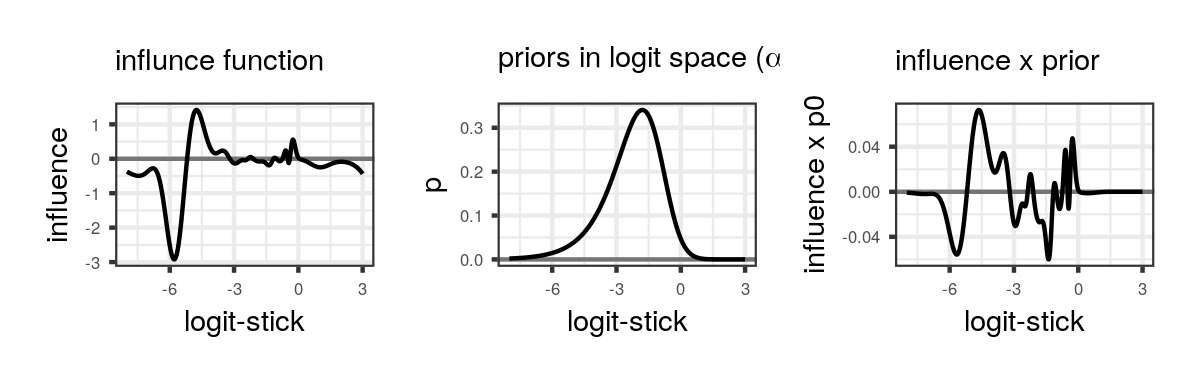
\includegraphics[width=0.980\linewidth,height=0.314\linewidth]{figure/gene_alpha_coclustering_influence-1} 

}

\caption[The influence function of $g_{ev}$, the sum of the eigenvalues of the coclustering Laplacian matrix]{The influence function of $g_{ev}$, the sum of the eigenvalues of the coclustering Laplacian matrix. }\label{fig:gene_alpha_coclustering_influence}
\end{figure}


\end{knitrout}





\begin{knitrout}
\definecolor{shadecolor}{rgb}{0.969, 0.969, 0.969}\color{fgcolor}\begin{figure}[!h]

{\centering 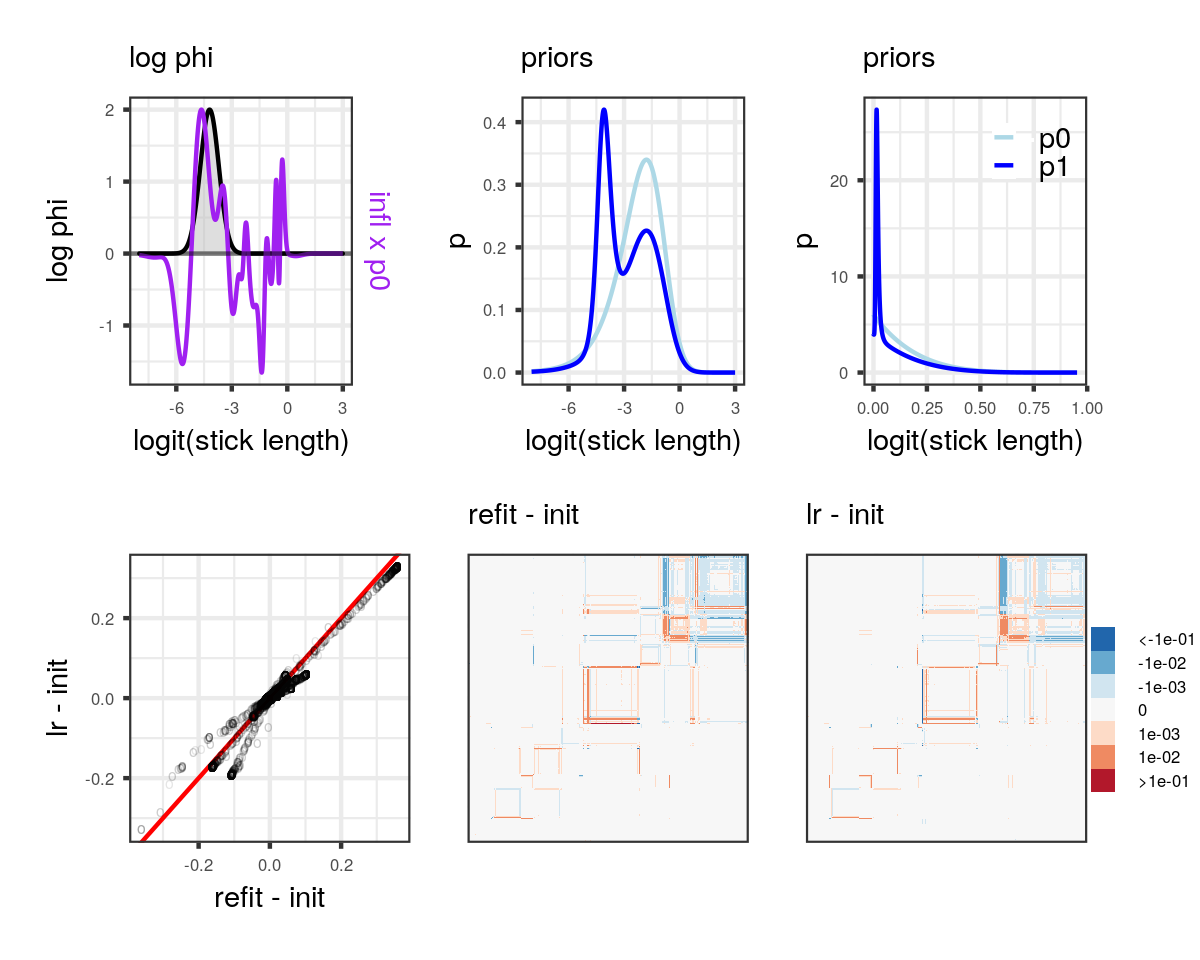
\includegraphics[width=0.980\linewidth,height=0.784\linewidth]{figure/gene_fpert_coclustering-1} 

}

\caption[Effect on the co-clustering matrix after a functional perturbation.
     log-phi (top left, in grey) is set to a Gaussian p.d.f]{Effect on the co-clustering matrix after a functional perturbation.
     log-phi (top left, in grey) is set to a Gaussian p.d.f. centered at mu = -4.2, and scaled to have L-infinity norm equal to two.
    The chosen log-phi roughly corresponds to a positive bump in the influence function of $g_{ev}$.}\label{fig:gene_fpert_coclustering}
\end{figure}


\end{knitrout}



\begin{knitrout}
\definecolor{shadecolor}{rgb}{0.969, 0.969, 0.969}\color{fgcolor}\begin{figure}[!h]

{\centering 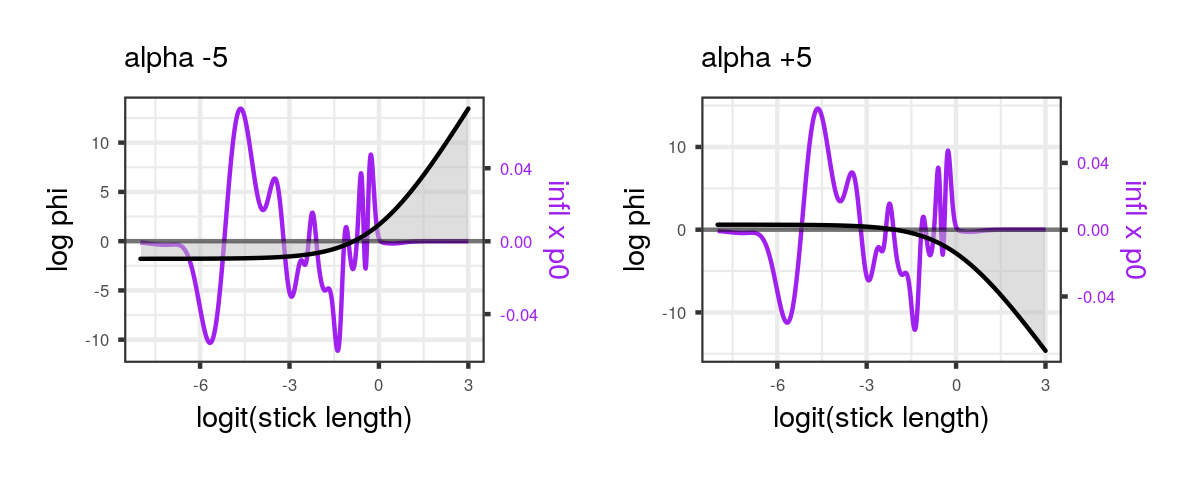
\includegraphics[width=0.980\linewidth,height=0.392\linewidth]{figure/alpha_pert_logphi-1} 

}

\caption[The log multiplicative perturbation $\log \phi$ corresponding to decreasing the $\alpha$ parameter by five (left) or increasing the $\alpha$ parameter by five (right)]{The log multiplicative perturbation $\log \phi$ corresponding to decreasing the $\alpha$ parameter by five (left) or increasing the $\alpha$ parameter by five (right). }\label{fig:alpha_pert_logphi}
\end{figure}


\end{knitrout}


\begin{table}[tb]
\centering
\caption{Compute time of results on the mice dataset. }
\begin{tabular}{|r|r|}
    \hline 
    & time (seconds) \\ 
    \hline 
    Initial fit & 35 \\
    \hline 
    Hessian solve for $\alpha$ sensitivity & 
        2.6\\
    Linear approx. $\eta^{lin}(\alpha)$ for $\alpha = 1$ & 
        0.0013\\
    Linear approx. $\eta^{lin}(\alpha)$ for $\alpha = 11$ & 
        0.0012\\
    Refit $\eta(\alpha)$ for $\alpha = 1$ & 
        12\\
    Refit $\eta(\alpha)$ for $\alpha = 11$ & 
        11\\
    \hline
    The influence function & 4.5\\ 
    Hessian solve for $\phi$ perturbation &
        4.9\\
    Linear approx. $\eta^{lin}(\epsilon)$ at $\epsilon = 1$ &
        0.001\\
    Refit $\eta(\epsilon)$ at $\epsilon = 1$ &
        14\\
    \hline
\end{tabular}
\end{table}
